\documentclass[12pt]{article}
\usepackage{tikz}
\usepackage{amsmath}
% Underlining package
\usepackage{ulem}
\usetikzlibrary{calc}
\usepackage[a4paper, portrait, margin=1cm]{geometry}
\usepackage{fancyhdr}

\def \HeadingAnswers {\section*{\Large Name: \underline{\hspace{8cm}} \hfill Date: \underline{\hspace{3cm}}} \vspace{-3mm}
{Coordinates: Answers} \vspace{1pt}\hrule}

% raise footer with page number; no header
\fancypagestyle{myfancypagestyle}{
  \fancyhf{}% clear all header and footer fields
  \renewcommand{\headrulewidth}{0pt} % no rule under header
  \fancyfoot[C] {\thepage} \setlength{\footskip}{14.5pt} % raise page number allowed min 14.5pt
}
\pagestyle{myfancypagestyle}  % apply myfancypagestyle

\newcounter{minipagecount}

\begin{document}
\HeadingAnswers

\bigskip
Write the x and y values of each point on the coordinate plane.

\bigskip

\begin{center}
  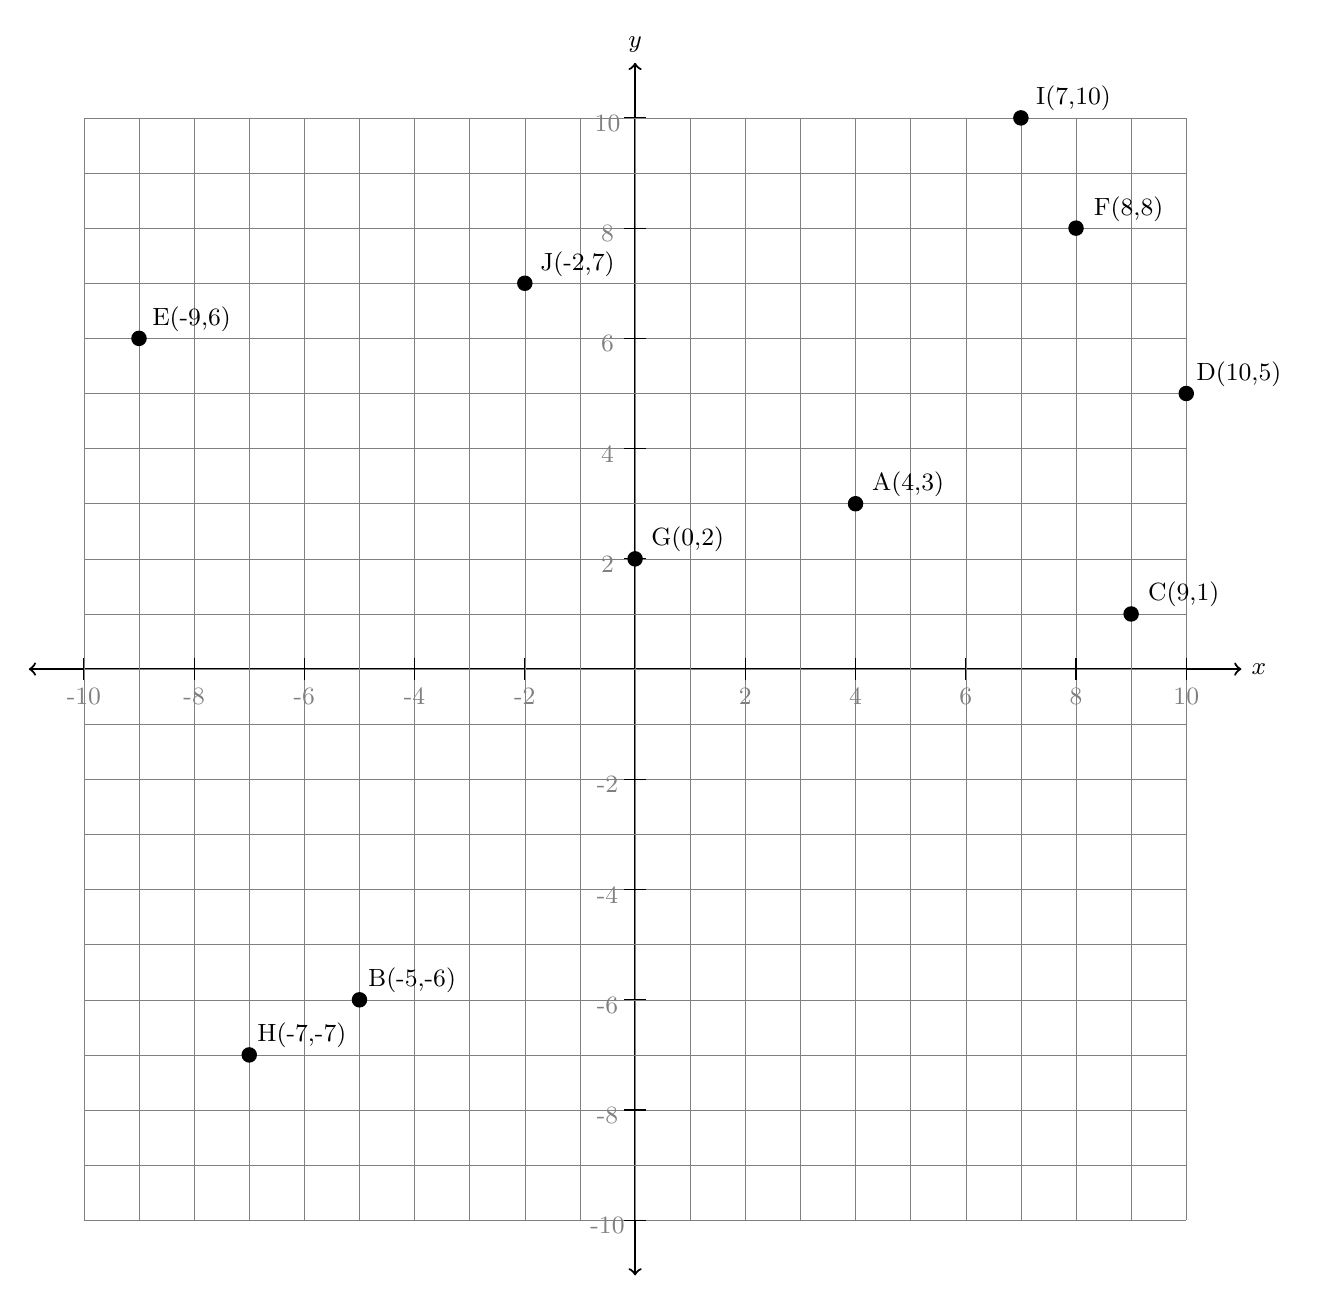
\begin{tikzpicture}[scale=0.7]
      % Draw axes
      \draw[thick,<->] (-11,0) -- (11,0) node[right] {\small $x$};
      \draw[thick,<->] (0,-11) -- (0,11) node[above] {\small $y$};

      % Grid
      \draw[very thin,gray] (-10,-10) grid (10,10);

      % Axis numbering (every second number, light gray)
      \foreach \x in {-10,-8,-6,-4,-2,2,4,6,8,10} {
          \draw (\x,-0.2) -- (\x,0.2);
          \node[gray] at (\x,-0.5) {\small \x};
      }
      \foreach \y in {-10,-8,-6,-4,-2,2,4,6,8,10} {
          \draw (-0.2,\y) -- (0.2,\y);
          \node[gray] at (-0.5,\y-0.1) {\small \y};
      }

    \fill (4,3) circle (4pt);
\node[xshift=1.9em, yshift=7pt] at (4,3) {\small A(4,3)};
\fill (-5,-6) circle (4pt);
\node[xshift=1.9em, yshift=7pt] at (-5,-6) {\small B(-5,-6)};
\fill (9,1) circle (4pt);
\node[xshift=1.9em, yshift=7pt] at (9,1) {\small C(9,1)};
\fill (10,5) circle (4pt);
\node[xshift=1.9em, yshift=7pt] at (10,5) {\small D(10,5)};
\fill (-9,6) circle (4pt);
\node[xshift=1.9em, yshift=7pt] at (-9,6) {\small E(-9,6)};
\fill (8,8) circle (4pt);
\node[xshift=1.9em, yshift=7pt] at (8,8) {\small F(8,8)};
\fill (0,2) circle (4pt);
\node[xshift=1.9em, yshift=7pt] at (0,2) {\small G(0,2)};
\fill (-7,-7) circle (4pt);
\node[xshift=1.9em, yshift=7pt] at (-7,-7) {\small H(-7,-7)};
\fill (7,10) circle (4pt);
\node[xshift=1.9em, yshift=7pt] at (7,10) {\small I(7,10)};
\fill (-2,7) circle (4pt);
\node[xshift=1.9em, yshift=7pt] at (-2,7) {\small J(-2,7)};

    

  \end{tikzpicture}
\end{center}\pagebreak ~ \newline ~ \newline\bigskip
Write the x and y values of each point on the coordinate plane.

\bigskip

\begin{center}
  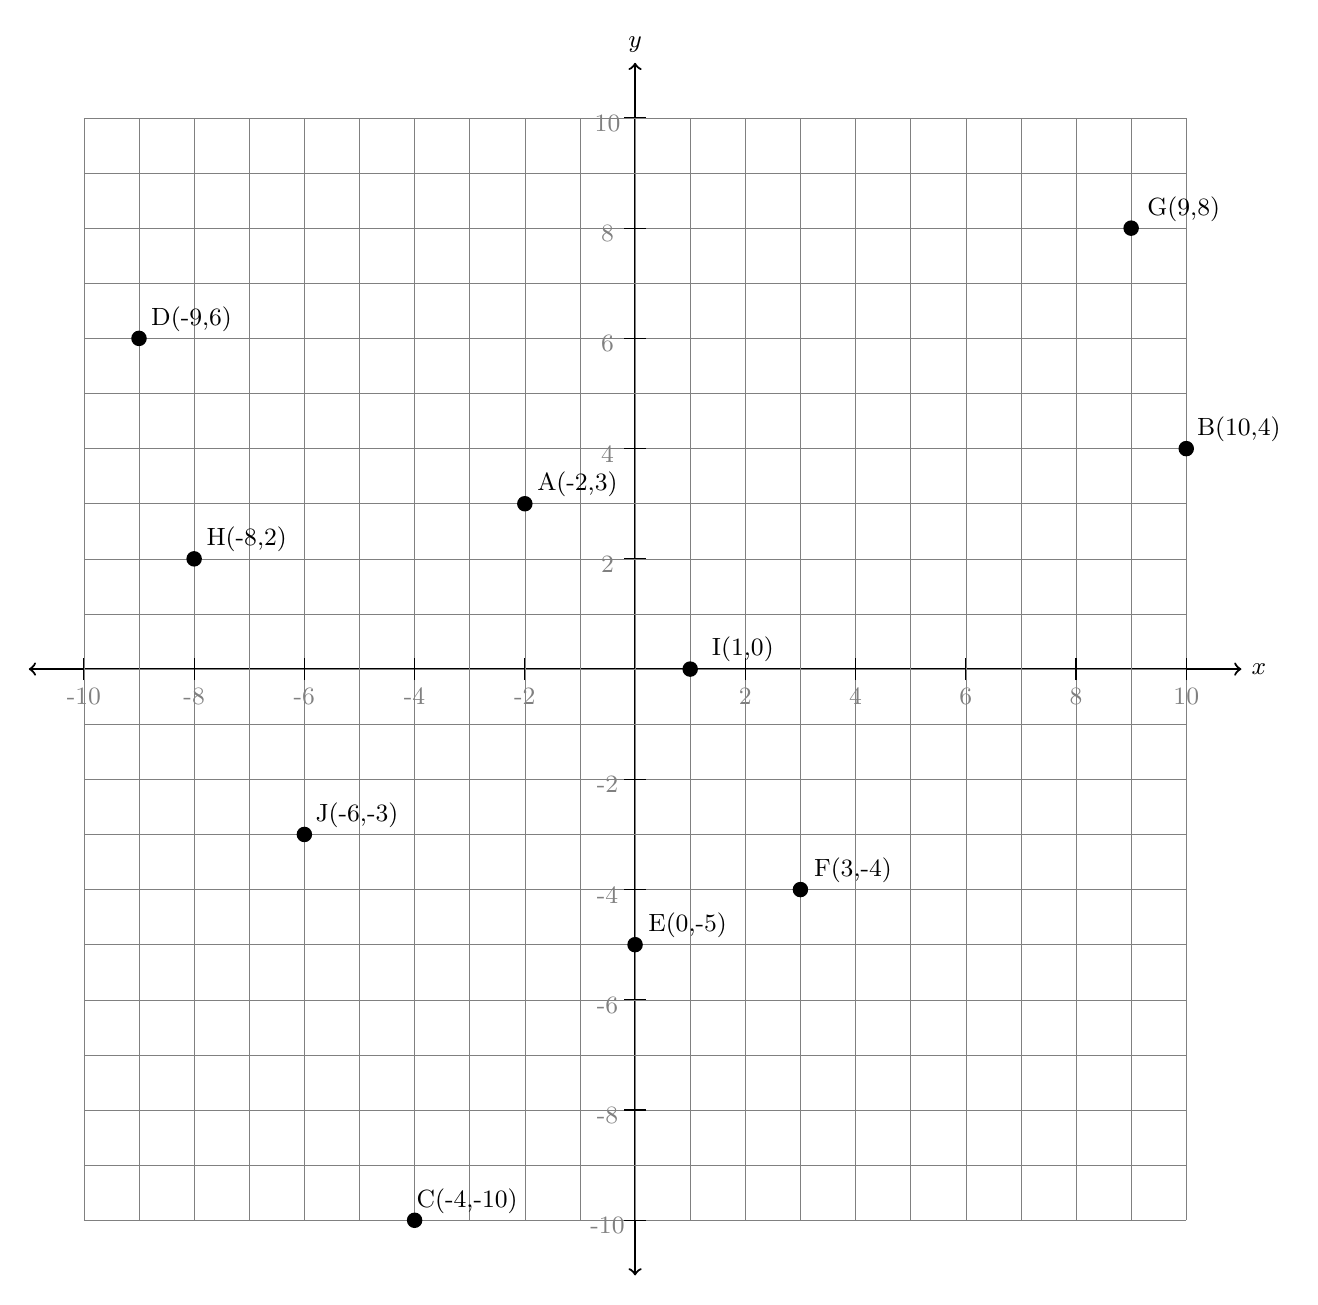
\begin{tikzpicture}[scale=0.7]
      % Draw axes
      \draw[thick,<->] (-11,0) -- (11,0) node[right] {\small $x$};
      \draw[thick,<->] (0,-11) -- (0,11) node[above] {\small $y$};

      % Grid
      \draw[very thin,gray] (-10,-10) grid (10,10);

      % Axis numbering (every second number, light gray)
      \foreach \x in {-10,-8,-6,-4,-2,2,4,6,8,10} {
          \draw (\x,-0.2) -- (\x,0.2);
          \node[gray] at (\x,-0.5) {\small \x};
      }
      \foreach \y in {-10,-8,-6,-4,-2,2,4,6,8,10} {
          \draw (-0.2,\y) -- (0.2,\y);
          \node[gray] at (-0.5,\y-0.1) {\small \y};
      }

    \fill (-2,3) circle (4pt);
\node[xshift=1.9em, yshift=7pt] at (-2,3) {\small A(-2,3)};
\fill (10,4) circle (4pt);
\node[xshift=1.9em, yshift=7pt] at (10,4) {\small B(10,4)};
\fill (-4,-10) circle (4pt);
\node[xshift=1.9em, yshift=7pt] at (-4,-10) {\small C(-4,-10)};
\fill (-9,6) circle (4pt);
\node[xshift=1.9em, yshift=7pt] at (-9,6) {\small D(-9,6)};
\fill (0,-5) circle (4pt);
\node[xshift=1.9em, yshift=7pt] at (0,-5) {\small E(0,-5)};
\fill (3,-4) circle (4pt);
\node[xshift=1.9em, yshift=7pt] at (3,-4) {\small F(3,-4)};
\fill (9,8) circle (4pt);
\node[xshift=1.9em, yshift=7pt] at (9,8) {\small G(9,8)};
\fill (-8,2) circle (4pt);
\node[xshift=1.9em, yshift=7pt] at (-8,2) {\small H(-8,2)};
\fill (1,0) circle (4pt);
\node[xshift=1.9em, yshift=7pt] at (1,0) {\small I(1,0)};
\fill (-6,-3) circle (4pt);
\node[xshift=1.9em, yshift=7pt] at (-6,-3) {\small J(-6,-3)};

    

  \end{tikzpicture}
\end{center}

\end{document}
